% 2009 年江苏卷第 13 题：椭圆的四个顶点、右焦点 F、交点 T 与中点 M。
% 来源 PDF：普通高考/2009/2009江苏.pdf
% SHA-256：64e417d45911d88d77c047a419dcc259e7c7dc779c79d20df2092755c96a4501
% 原页：2009江苏.pdf 第 1 页（A3 三栏）第 2 栏，书页码 531。
% 绘制依据：按原页画椭圆 A1A2B2B1、右焦点 F、直线 A1B2 与 B1F 的交点 T，
%   以及 OT 的中点 M（落在椭圆上）；示意取 a=2.6，b≈2.487，e=2√7−5。
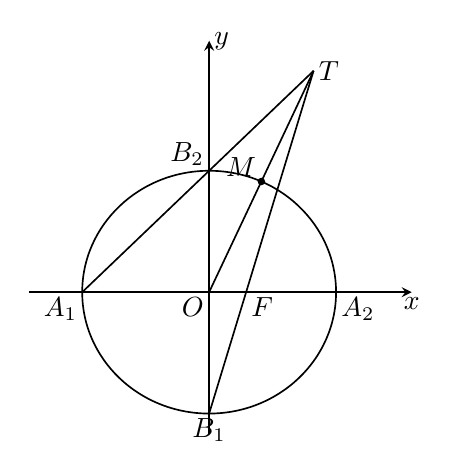
\begin{tikzpicture}[scale=0.62, semithick, every node/.style={inner sep=1.6pt}]
  \draw (0,0) ellipse [x radius=2.6, y radius=2.4868];

  \coordinate (A1) at (-2.6,0);
  \coordinate (A2) at (2.6,0);
  \coordinate (B1) at (0,-2.4868);
  \coordinate (B2) at (0,2.4868);
  \coordinate (F) at (0.7579,0);
  \coordinate (T) at (2.1394,4.5335);
  \coordinate (M) at (1.0697,2.2668);

  \draw[->,>=stealth] (-3.7,0) -- (4.15,0) node[below] {$x$};
  \draw[->,>=stealth] (0,-2.9) -- (0,5.15) node[right] {$y$};

  \draw (A1) -- (T);
  \draw (B1) -- (T);
  \draw (0,0) -- (T);

  \fill (M) circle (2.2pt);

  \node[below left] at (A1) {$A_1$};
  \node[below right] at (A2) {$A_2$};
  \node[below] at (B1) {$B_1$};
  \node[above left] at (B2) {$B_2$};
  \node[below right] at (F) {$F$};
  \node[right] at (T) {$T$};
  \node[above left] at (M) {$M$};
  \node[below left] at (0,0) {$O$};
\end{tikzpicture}
